\begin{displayquote}
	\textsf{Many problems in science and engineering often require to solve a long sequence of large-scale non-Hermitian linear systems with different Right-hand sides (RHSs) but a unique operator. Efficiently solving such problems on extreme-scale platforms requires the minimization of global communications, reduction of synchronization points and promotion of asynchronous communications. Unite and Conquer GMRES/LS-ERAM (UCGLE) method presented in the last chapter is a suitable candidate with the reduction of global communications and the synchronization points of all computing units. In this chapter, we extend both the mathematical model and the implementation of UCGLE method to adapt to solve sequences of linear systems. The eigenvalues obtained in solving previous linear systems by UCGLE can be recycled, improved on the fly and applied to construct a new initial guess vector for subsequent linear systems, which can achieve a continuous acceleration to solve linear systems in sequence. Numerical experiments using different test matrices to solve sequences of linear systems on supercomputer Tianhe-2 indicate a substantial decrease in both computation time and iteration steps when the approximate eigenvalues are recycled to generate the initial guess vectors.}
\end{displayquote}
 
\vspace{0.6in}

\section{Demand to Solve Linear Systems in Sequence}

We consider the solution of a long sequence of general linear systems 

\begin{equation}
Ax^{(i)}=b^{(i)}, i=1,2,\cdots
\end{equation}

where $A \in \mathbf{C}^{n\times n}$ is a fixed matrix, and the right-hand side $b^{i} \in \mathbf{C}^n$ which changes from one system to another. Moreover, these systems are typically not available simultaneously. Many scientific applications require the resolution this kind of sequent linear systems, such as the finite element analysis in modeling fatigue \cite{newman1976finite, gullerud2001mpi,sukumar2003extended}, diffuse optical tomography \cite{kilmer2006recycling,arridge1993finite,schweiger1995finite}, electromagnetic \cite{bastos2003electromagnetic,pridmore1981investigation, ye2008generalized} and wave-propagation for the earthquake simulation \cite{Fujita:2018:WPS:3149457.3149474,moczo2007finite,chen2015transient}, etc. Generally, these systems are formatted by the time-dependent applications, where the operator matrix $A$ keeps the same, but the right-hand side $b^{(i)}$ cannot be gotten in the same time. In many fields, the next right-hand side of the linear system depends on the previous solution. Thus only one linear system is available at a time. Another application of these sequent linear systems are the Newton methods for solving nonlinear equations (e.g., \cite{brown1990hybrid,knoll2004jacobian,bellavia2001globally,flueck1998solving,an2007globally}). 

If the direct solvers are applicable, their decompositions can be shared and reused for the successive linear systems by the forward/backward solves. When the matrix has a large dimension or special sparsity pattern, and the direct solvers are not applicable, then the iterative methods based on Krylov subspace, such as CG (Conjugate Gradient) method \cite{kershaw1978incomplete} for symmetric systems, and GMRES (Generalized minimal residual ) method \cite{saad1986gmres} for non-Hermitian systems, are considerable. Obviously, this naive implementation is not efficient enough, since the sequence of linear systems shares the same matrix $A$. The intermediate information computed from the previous system's solution can be reused to speed up the solution of the next systems. There are already several methods proposed to take advantage of this temporary information in order to speed up resolving the sequences of linear systems. The first approach is to use the seed methods (e.g., \cite{saad1987lanczos,papadrakakis1990new,smith1989conjugate,gu2002seed,simoncini1995iterative,abdel2014improved}). This method selects one seed system and solve it by the Krylov iterative method, and then a Galerkin projection of the other right-hand sides is performed onto the Krylov subspace generated by the seed system. It is efficient since the Krylov subspace generated by the previous time resolution develops a good approximation to the eigenvectors of small eigenvalues of $A$, and the projection of the other right-hand sides over this subspace can remove the components of their residual vectors in the directions these eigenvectors. The seed method requires more memory space to store the subspace of seed systems. The speedup cannot always be guaranteed for the uncorrelated right-hand sides.  It can also be inefficient for the restarted methods, in this case, even the convergence of resolving the seed systems maybe stagne. Another approach is to improve the convergence for a sequence of linear systems by the process of Krylov Subspace Recycling (e.g. \cite{parks2006recycling,jolivet2016block,kilmer2006recycling,ye2008generalized}). For example, by recycling the Krylov subspace generated by previous resolution, the method GCRO-DR (Generalized Conjugate Residual method with inner Orthogonalization
and Deflated Restarting) proposed by M.L. Parks \cite{parks2006recycling} allows to speed up the solution of systems from one right-hand side to another or even between two times restart of iterative methods through the maintain of the Arnoldi subspace orthogonalization and the deflation of smallest eigenvalues. Additionally, Block iterative methods are a popular way to solve systems with multiple-right hands (e.g., \cite{simoncini1995iterative,calvetti1994application, baker2006improving,gutknecht2006block}), but the different right-hand sides should simultaneously known, which is not the exact case talked in this paper. 

\section{Existing Methods and Analysis}
\subsection{Seeds Method}

\textcolor{red}{This section needs analyze in details the seeds method, espacially the unstability for uncorrelerated RHSs.}

Algorithm \ref{alg:seed_gmres} gives one kind of implementation of seeds method.

\begin{algorithm}[htbp]{}
	\caption{The seed-GMRES algorithm}   
	\label{alg:seed_gmres}   
	\begin{algorithmic}[1]
		\State Choose $n_{max}$, the maximum size of the subspace. For each RHS $b^{(l)}$, choose an initial guess $x_0^{(l)}$ and compute $r_0^{(l)} = b^{(l)}-Ax_0^{(l)}$. The recast problem is the error system $A(x^{(l)}-x_0^{(l)})=r_0^{(l)}$, choose a RHS $k$, the first on which a cycle of GMRES is applied. Set $Z_p=(z_1,\cdots, z_p)$, $p$ vectors of size $m$, to zero.
		\State run one cycle of GMRES($n_{max}$) on $r_0^{(k)}$, either it converges in $n=n_1$ step or stops after $n=n_{max}$ steps. This GMRES provides us with $V_{n+1}$, that has orthonormal columns, and $\underline{H}_{n+1,n}$ such that $AV_n=V_{n+1}\underline{H}_{n+1,n}$. The approximate solution for the $k$-th system writes $x_n=x_0^{(k)}+MV_ny_n^{(k)}$ but is not computed as such. The vector $z_k$ is updated via $z_k=z_k+V_ny_n^{(k)}$ and the residual can be formatted via $x^{(k)}=x_0^{(k)}+Mz_k$. If all the systems have converged, stop.
		\State For each RHS $L \neq k$ that has not converged, form $c^{(l)}= V_{n+1}^Tr_0^{(l)}$ and compute $y_n^{(l)}$ the solution of the least squares problems $||\underleftarrow{H}_{n+1,n}y-c^{(l)}||_2$. Compute $z_l=z_l+V_ny_n^{(l)}$ and the residual $r_n^{(l)}=(I_m-V_{n+1}V_{n+1}^T)r_0^{(l)}+V_{n+1}(c^{(l)}-\underleftarrow{H}_{n+1,n}y_n^{(l)})$. If the system has $l$ converged, form the approximate solution $x^{(l)}=x_0^{(l)}+Mz_l$. If all the systems have converged, stop.
		\State For each RHS $l$ that has not converged, set $r_0^{(l)}=r_n^{(l)}$. Choose a vector to run a cycle of GMRES. Traditionaly we take the first $l$ in the list $k, k+1, \cdots p$, so that the system $l$ has not converged and go to step $2$. 
	\end{algorithmic}  
\end{algorithm}

\subsection{Krylov Subspace Recycling Methods}

\textcolor{red}{This section gives an example as GCR-DO, anaylze the synchronization points, etc.}

The workflow of GCR-DO is given in Fig. \ref{fig:gcrdo}.

\begin{figure}[htbp]
	\centering
	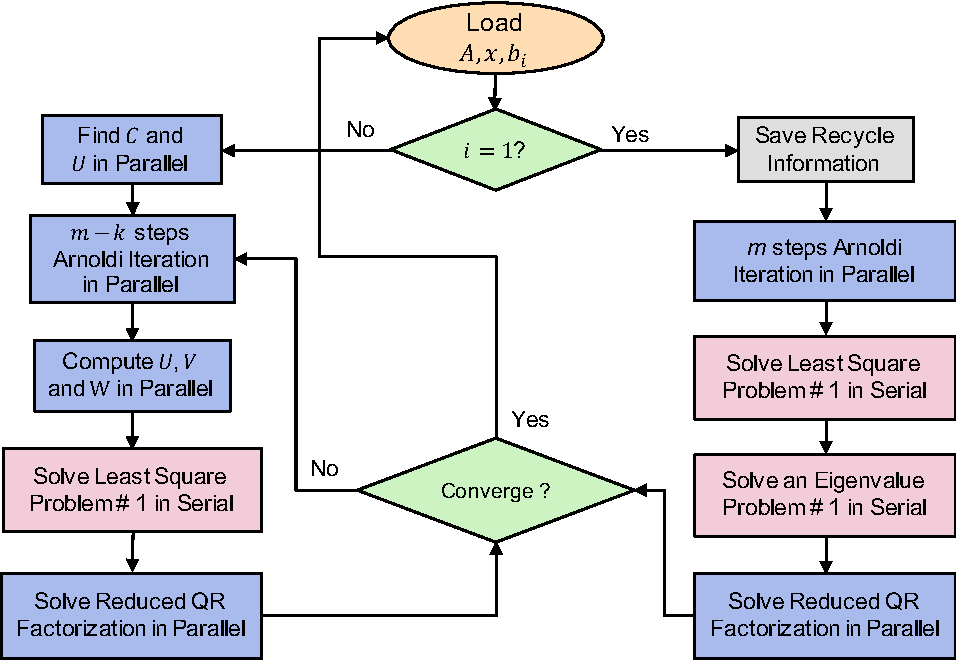
\includegraphics[width=5.in]{fig/gcrdo.pdf}
	\caption{GCR-DO workflow.}
	\label{fig:gcrdo}
\end{figure}

\subsection{Challenges of Exising Methods}

\textcolor{red}{TO DO}

\section{UCGLE method for Linear Systems with Sequent Right-hand-sides}

In this section, we introduce another point of view to solve sequences of non-Hermitian linear systems for modern computer architectures, based on UCGLE method. Inside of UCGLE, the dominant eigenvalues are used to accelerate the convergence of iterative methods. The more the eigenvalues are calculated, the more accurate these values are, the more significant the acceleration will be. When using UCGLE to solve the sequences of linear systems, the eigenvalues computed during the previous resolution can be reused, and sometimes improved, to resolve the following sequences of different linear systems. Theoretically, the continuous amelioration of convergence for the rest of the linear systems can be achieved. Moreover, the eigenvalues computed from the previous resolution can be used to construct an approximative solution by LS method and serve as an initial guess vector to speedup up the next time resolution.

\subsection{Relation between LS Residual and Dominant Eigenvalues}

Suppose that the computed convex hull by Least Squares contains eigenvalues $\lambda_1,\cdots, \lambda_m$, the residual given by Least Squares polynomial of degree $d-1$ is

\begin{equation}
\label{rnk3}
r = \sum_{i=1}^{k}\rho_i (R_d(\lambda_i))^l u_i + \sum_{i=m+1}^{n}\rho_i (R_d(\lambda_i))^l u_i,
\end{equation}

this residual can be divided into two parts. The first part is formulated with the first known $m$ eigenvalues which are used to computed the convex hull by LS Component, the second part represents the residual with unknown eigenpairs.

\begin{figure}[htbp]
	\centering
	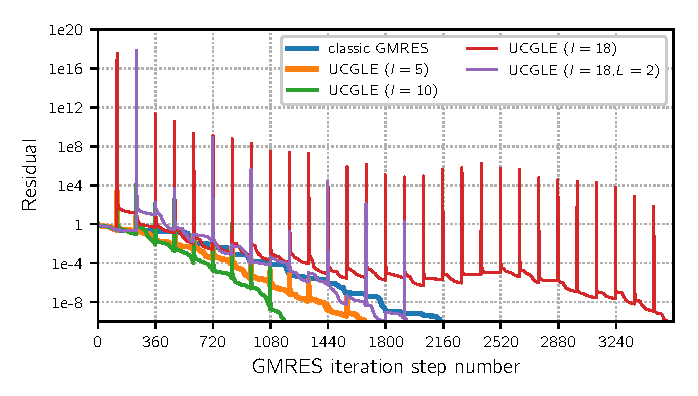
\includegraphics[width=6.2in]{fig/conv2.eps}
	\caption{Convergence comparison of UCGLE method vs classic GMRES.}
	\label{fig:convg}
\end{figure}

In practice, for each time preconditioning by LS polynomial method, it is often repeated for several times to improve its acceleration of convergence, that is the meaning of parameter $l$ in Equation (\ref{rnk3}). The LS polynomial preconditioning applies $r_d$ as a deflation vector for each time GMRES restart process. Fig. \ref{fig:conv} gives the comparison between classic GMRES and UCGLE with different values for the parameter $l$. As shown in this figure, the first part in Equation (\ref{rnk3}) is small since the LS method finds $R_d$ minimizing $|R_d(\lambda)|$ in the convex hull, but not with the second part, where the residual will be rich in the eigenvectors associated with the eigenvalues outside $H_k$. As the number of approximated eigenvalues $k$ increasing, the first part will be much closer to zero, but the second part keeps still large. This results in an enormous increase of restarted GMRES preconditioned vector norm. Meanwhile, when GMRES restarts with the combination of a number of eigenvectors, the convergence will be faster even if the residual is enormous, and the convergence of GMRES can still be significantly accelerated. The peaks are shown in Fig. \ref{fig:convg} for each time restart of UCGLE represent these enormous residuals. The $l$ times repeat of $r_d$ before applying to next time restart can still enlarge its norm, and the selection of $l$ is important for the acceleration. In the example of Fig. \ref{fig:convg}, we conclude that if $l$ is too large, the norm trends enormous, which slows down the speedup, if $l$ is small, the acceleration may not be evident. In some situation, the preconditioned residual may be too large, and it results that GMRES cannot converge enough before the next restart. Hence the LS preconditioning can be applied each $L$ times of GMRES restart, and the best $l$ should be found.

\subsection {Eigenvalues Recycling to Solve Linear Systems in Sequence}

After the analysis of relation between LS polynomial residual and the approximated eigenvalues, it is apparent that these dominant eigenvalues used by LS Component to accelerate the convergence, can be recycled and improved from the procedure of solving system with one RHS to another, which will introduce a potential continuous improvement for solving a long sequence of linear systems.

In order to solve the sequence of linear systems $Ax= b_t$ with $t \in 1,2,3, \cdots$. We enlarge the Krylov subspace size $m_a$ inside ERAM Component to approximate more eigenvalues. Suppose that $(m_a)_1$ for the first system, the exact implementation of ERAM Component for $t \in 2,3, \cdots$ is shown in Equation (\ref{rnk2}), $(m_a)_t$ is equal to the sum of $(m_a)_{t-1}$ and a given constant $a$. And $k_t$, the number of eigenvalues computed by ERAM Component for $Ax=b_t$ can be described by a function $f$ which maps the relation between $(m_a)_t$ and $k_t$. Obviously, $k_t \geq k_{t-1}$. The residual $(r_d)_t$ for each restart of $Ax=b_t$ with $t \in 2,3, \cdots$ is also given in (\ref{rnk2}).
\begin{equation}
\label{rnk2} \left \{
\begin{aligned}
(m_a)_t &=  (m_a)_{t-1}+a\\
k_t &= f(m_t) \\
(r_d)_t =\sum_{i=1}^{k_t}(R_d(\lambda_i))^l &\rho_i u_i + \sum_{i=k_t+1}^{n}(R_d(\lambda_i))^l \rho_i u_is \\
\end{aligned}
\right.
\end{equation}

With the enlargement of ERAM Component Krylov subspace size, the more eigenvalues are calculated, then the first part of $(r_d)_t$ in Equation (\ref{rnk2}) are more important, and the more significant the  acceleration will be. The continuous amelioration of convergence for solving linear systems in sequence can be gotten. With the changing of ERAM component Krylov subspace size, it may not be guaranteed to get the demanded eigenvalues in time for each restart of GMRES component if this size is too large comparing with GMRES Component Krylov subspace size. In order to improve the robustness of UCGLE, the previously calculated eigenvalues are kept in memory and updated if there come the new ones. These values in memory can be utilized in case that the failure of ERAM component when the parameters are too strict. In Equation (\ref{rnk2}), we did not define the upper limit for $(m_a)_t$, which depends on properties of operator matrices and $P_g$ and $P_a$ for GMRES and ERAM components. 

For $t \in 2,3, \cdots$, since the eigenvalues calculated when solving $Ax = b_{t-1}$ are kept in memory, they can be used to construct an approximative solution for the current linear system $Ax=b_t$ through the LS polynomial method before its solve by GMRES. Obviously, this approximative solution can be used as a non-zero initial guess vector $(x_0)_t$ to solve $Ax=b_t$. It will introduce an acceleration on the convergence for solving the linear systems in sequence. With the number of linear systems to be solved increasing, there will be more eigenvalues approximated, the initial guess vector constructed by LS component will be more accurate, and thus the speedup for solves from one to another can be still gotten. In fact, the impact of initial guess vector on the convergence is different from the restarted residual vector inside the iterative method, we propose a new parameter $l'_t$ for the initial guess generation procedure which is different from the $l$ in LS preconditioning part. The residual vector $(g_d)_t$ for $Ax=b_t$ with $t \in 2,3, \cdots$ is given in Equation (\ref{rnk4}), which is constructed  by the $k_{t-1}$ number of eigenvalues calculated when solving $Ax=b_{t-1}$.

\begin{equation}
\label{rnk4}
(g_d)_t=\sum_{i=1}^{k_{t-1}}(R_d(\lambda_i))^{l'_t} \rho_i u_i + \sum_{i=k_{t-1}+1}^{n}(R_d(\lambda_i))^{l'_t} \rho_i u_i.
\end{equation}

In this section, two parameters are added in order to resolve linear systems in sequence using UCGLE, they are listed as below:

\begin{enumerate}
	\item $(m_a)_t$: ERAM Krylov subspace size for solving $Ax=b_t$
	\item $l'$: times that LS polynomial applied for the generation of initial guess vector
\end{enumerate}

It is predictable that this speedup for solving successive systems will stagnate after the optimized values of $m_a$ and $l'$ are found. It is useless to use ERAM Component to approximate the eigenvalues continuously. Thus $P_a$ computing units allocated for ERAM Component can be redistributed to GMRES Component. It is expected to get an extra speedup on the performance with more computing resources.

\begin{figure}[htbp]
	\centering
	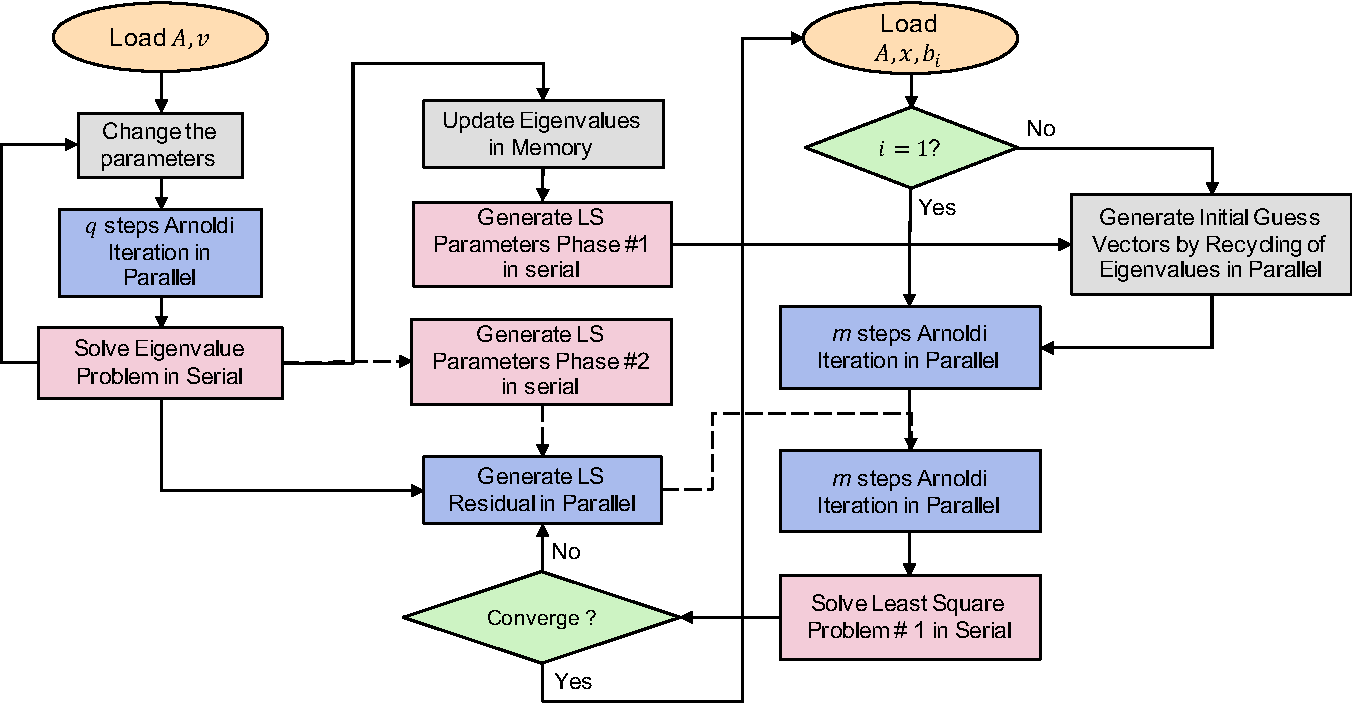
\includegraphics[width=6.2in]{fig/uclge_seq_workflow.pdf}
	\caption{Workflow of UCGLE to Solve Linear Systems In Sequence.}
	\label{fig:uclge_seq_workflow}
\end{figure}

The Algorithm \ref{alg:gmres_multi} gives the procedure of UCGLE for the resolution of a sequence of linear systems $Ax= b_t$ with $t \in 1,2,3, \cdots$. Initially, $P_g$ and $P_a$ are respectively set to be $proc_g$ and $proc_a$.  If $t=1$, UCGLE loads normally the three computation components with the ERAM component's Krylov subspace to be $(m_a)_1$, and the initial guess vector for GMRES component to be zero. For the resolution of the successive linear systems, before the update of three components, a $INITIAL\_GUESS$ function is performed which is the same as the LS component but with different parameter $l'$. The $INITIAL\_GUESS$ function will generate an initial guess vector ${g_d}_t$. Inside GMRES component, the initial guess vector is updated by ${g_d}_t$ before the start of resolution. Moreover, the Krylov subspace Size of ERAM Component is replaced by $(m_a)_t$. When the optimized values of $(m_a)_{op}$ and $l'_{op}$ are found, the eigenvalues are kept into a local file $eigenvalue.bin$. The $P_g$ and $P_a$ are respectively updated as  $proc_g+proc_a-1$ and $1$. The $INITIAL\_GUESS$ function executes by loading $eigenvalue.bin$. $LOADGMRES$ is restarted with the redeployment of its data onto $proc_g+proc_a-1$ computing units. $LS$ also executes with $eigenvalue.bin$. The retainment of $1$ computing unit for ERAM Component aims to ensure the distributed and parallel implementation of UCGLE with high fault tolerance. However, the inside kernel of ERAM Component is replaced by a simple function with keeping the data sending and receiving functionalities.

\begin{algorithm}
	\caption{UCGLE for sequences of linear systems}
	\label{alg:gmres_multi}
	\begin{algorithmic}[1]
		\For {($t \in (1,2,3,\cdots)$)}
		\If {($t=1$)}
		\State set $P_g = proc_g$ and $P_a=proc_a$
		\State $LOADERAM(input: A, m_a, v, r, \epsilon_a)$
		\State $LOADLS(input: A,b, d)$
		\State $LOADGMRES(input: A, m_g, x_0, b_1, \epsilon_g, L, l, output: x_m)$
		\Else
		\State set $P_g = proc_g$ and $P_a=proc_a$
		\State $INITIAL\_GUESS(input: A, b_t, d, output: {g_d}_t)$
		\State update $LOADGMRES(input: A, m_g, {g_d}_t, b_{t}, \epsilon_g, L, l, output: x_m)$
		\State update $(m_a)_{t-1}$ by $(m_a)_{t}$ in $LOADERAM(input: A, (m_a)_{t}, v, r, \epsilon_a)$
		\State update $LOADLS(input: A,b_{i}, d)$
		
		\If {(optmized $(m_a)_{op}$ and $l'_{op}$ found)}
		\State save the eigenvalues to $eigenvalues.bin$
		\State set $P_g = proc_g+proc_a - 1$ and $P_a=1$
		\State $INITIAL\_GUESS(input: A, b_t, d, output: {g_d}_t)$ by loading $eigenvalues.bin$
		\State $LOADGMRES(input: A, m_g, {g_d}_t, b_{t}, \epsilon_g, L, l'_{op}, output: x_m)$
		\State replace $LOADERAM$ by a simple useless function
		\State $LOADLS(input: A,b_{i}, d)$ by loading $eigenvalues.bin$
		\EndIf
		\EndIf
		\EndFor
	\end{algorithmic}
\end{algorithm}

\subsection{Experiments of UCGLE for Sequences of Linear Systems}

In this section, we evaluate the UCGLE for solving the sequences of linear systems on the supercomputer using different generated test matrices. UCGLE with or without initial guess vector generation is compared with conventional restarted GMRES with or without available preconditioners (Jacobi and SOR) in our implementations. The parallel performance on different homogeneous and heterogeneous platforms is presented in \cite{Wu:2018:DPA:3149457.3154481}. Thus this paper concentrates on the numerical performance of UCGLE for solving non-Hermitian linear systems in sequence, and the parallel performance comparison will not be discussed. Indeed, the performance of UCGLE can achieve further improvement with unique implementation targeting at different computer architectures, but this is not the purpose of this paper. \textit{Unite and Conquer approach} (including UCGLE) is a particular programming model which introduces a better performance on top of classic solvers and makes them be more suitable for modern computers. It is fair to prove the benefits of \textit{Unite and Conquer approach} by comparing it with the implementations of classic solvers based on the same basic operations (distribution of matrix across the cores, parallel sparse matrix-vector operation, the orthogonalization in Arnoldi reduction, etc.) without specific optimization for different platforms. In fact, if we optimize the parallel implementation of classic solvers and also the components (especially GMRES Component) in UCGLE at the same time, the benefits of UCGLE by reducing the global communications and promoting the asynchronization are still there.  

\subsubsection{Experimental Hardwares}

UCGLE is implemented on the supercomputer \textit{Tianhe-2}, installed at the National Super Computer Center in Guangzhou of China. It is a heterogeneous system made of Intel Xeon CPUs and Matrix2000, with 16000 compute nodes in total. Each node composes 2 Intel Ivy Bridge 12 cores @ 2.2 GHz. In this paper, we did not test UCGLE with co-processor Matrix2000 on \textit{Tianhe-2} since our implementation does not support it with good performance. 

\subsubsection{Experimental Results}

We evaluate UCGLE for solving sequences of linear systems using three test matrices of size $1.572\times10^7$ generated by SMG2S with different given spectra. They are respectively denoted as $Mat1$, $Mat2$ and $Mat3$. The different right-hand sides of these sequent linear systems are generated at random. The parameter $l$ for all tests using UCGLE keeps the same as $10$. The numbers of process for GMRES and ERAM Components in UCGLE are respectively $768$ and $384$. Five methods are compared in the experiments, and the notations of different methods are given as below:

\begin{itemize}
	\item GMRES: classic restarted GMRES;
	\item GMRES+SOR or SOR: GMRES with SOR preconditioner;
	\item GMRES+Jacobi or Jacobi: GMRES with Jacobi preconditioner;
	\item UCGLE without initial guess: UCGLE without using previously obtained eigenvalues to generate an initial guess vector for the next system by LS polynomial method;
	\item UCGLE with initial guess: UCGLE using previously obtained eigenvalues to generate an initial guess vector for the next systems by LS polynomial method.
\end{itemize}

ERAM and LS components in UCGLE demand additional computing units. It is unfair to test only the conventional methods of their numbers of CPUs equal to the number of GMRES components in UCGLE. Therefore, experiments have also been tested that the numbers of computing units of the classical iterative method are equal to the total CPU in UCGLE (hence, the CPUs for GMRES and ERAM components are included). In the captions of figures, a given method "with total CPUs" means that its number of CPUs equals the total CPU in UCGLE. The time comparisons for solving nine sequent linear systems of $Mat1$, $Mat2$ and $Mat3$ are given respectively in Fig. \ref{fig:seqrhs1} (a), Fig. \ref{fig:seqrhs3} (a) and Fig. \ref{fig:seqrhs2} (a), the comparison of the number of iteration for convergence are respectively given in Table 1, Table 2 and Table 3. From these three tables, we conclude that UCGLE can speed up the convergence to solve linear systems with test matrices comparing with the conventional methods. The generation of initial vectors using the eigenvalues for subsequent linear systems can still speed up the convergence over the UCGLE without initial guess.

\begin{table}[htbp]
	\small
	\label{tb1}
	\caption{$Mat1$: iterative step comparison for solving a sequence of linear systems.}
	\centering
	\renewcommand{\arraystretch}{1.6}
	\begin{tabular}{c*{9}{c}}
		\toprule
			\cellcolor{gray!50}Method              & \cellcolor{gray!50}1 &  \cellcolor{gray!50}2 &  \cellcolor{gray!50}3 &  \cellcolor{gray!50}4 &  \cellcolor{gray!50}5  &  \cellcolor{gray!50}6  & \cellcolor{gray!50}7 & \cellcolor{gray!50}8 & \cellcolor{gray!50}9\\
		\midrule
		GMRES & 509 & 505 & 501 & 505 & 527 & 510  &523&516& 518\\
			\cellcolor{gray!20}GMRES+SOR            & 	\cellcolor{gray!20}169 & 	\cellcolor{gray!20}165 & 	\cellcolor{gray!20}172 & 	\cellcolor{gray!20}130 & 	\cellcolor{gray!20}172 & 	\cellcolor{gray!20}173 &	\cellcolor{gray!20}130&	\cellcolor{gray!20}170&	\cellcolor{gray!20}130\\
		GMRES+Jacobi            & 274 & 273 & 270 & 276 & 269 & 274 &280&276&273\\
			\cellcolor{gray!20}UCGLE w/o initial guess     & 	\cellcolor{gray!20}120 & 	\cellcolor{gray!20}90 & 	\cellcolor{gray!20}90 & 	\cellcolor{gray!20}90 & 	\cellcolor{gray!20}90 &	\cellcolor{gray!20}90 &	\cellcolor{gray!20}90&	\cellcolor{gray!20}90& 	\cellcolor{gray!20}90\\
		UCGLE with initial guess     & 120 & 36 & 35 & 35 & 36 &36  &36&33&35\\
		\hline
	\end{tabular}
\end{table}

\begin{figure}
	\centering
	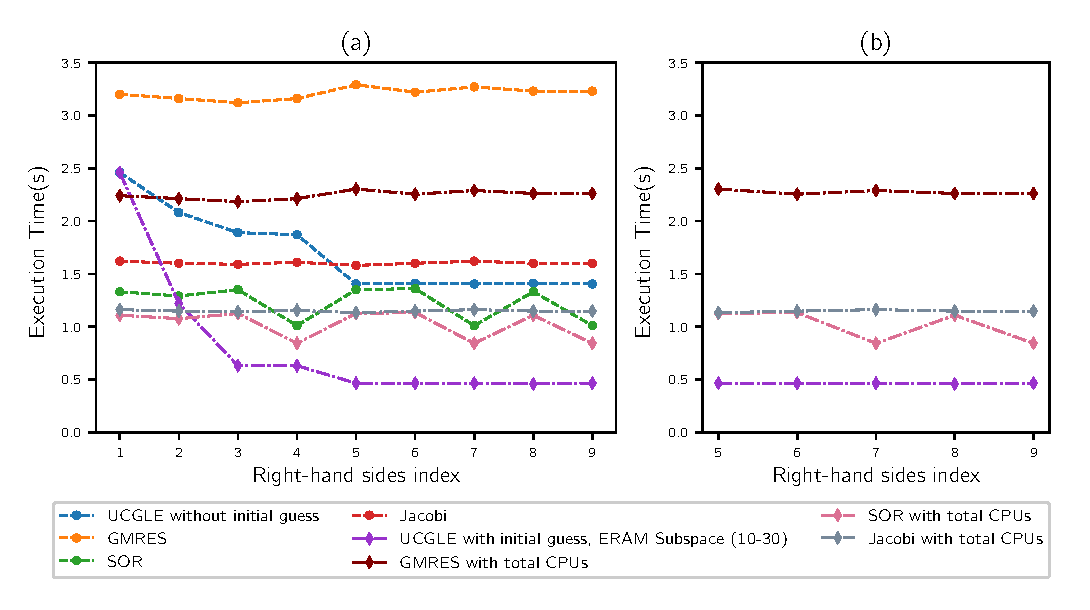
\includegraphics[width=6.4in]{fig/seqrhs1.eps}
	\caption{$Mat1$: time comparison for solving a sequence of linear systems. (a) shows the solution time for 9 sequent linear systems; (b) shows the cases extracted from (a) after the good selection of parameters in UCGLE.}
	\label{fig:seqrhs1}
\end{figure}

For the tests of $Mat1$, the GMRES restart size is $30$, the Krylov subspace of ERAM Component for solving the first three linear systems are respectively $10$, $20$ and $30$, the size of this subspace of ERAM for the remaining systems keeps being $30$. For the tests of $Mat2$, the GMRES restart size is $300$, the Krylov subspace of ERAM Component for solving the first three linear systems are respectively $100$, $150$ and $200$, the size of this subspace of ERAM for the remaining systems keeps being $200$. For the cases that UCGLE with initial guess, the parameter $l'$ for $Mat1$ and $Mat2$ keeps $30$. With the augmentation of the size of ERAM Krylov subspace, there will be more eigenvalues to be approximated, and we find that there is acceleration with the accumulation of more eigenvalues for both the case UCGLE with and without initial guess. The influence of subspace of ERAM can be found through the curves of UCGLE with/without initial guess in Fig. \ref{fig:seqrhs1} (a) and Fig. \ref{fig:seqrhs3} (a). However, it is not practical to enlarge too much the Krylov subspace of ERAM to approximated more eigenvalues, since if it is too large, it takes too much time by ERAM, LS Component cannot receive the eigenvalues in time, thus it will be difficult for the GMRES Component to perform the LS preconditioning for it each time restart.

\begin{figure}[htbp]
	\centering
	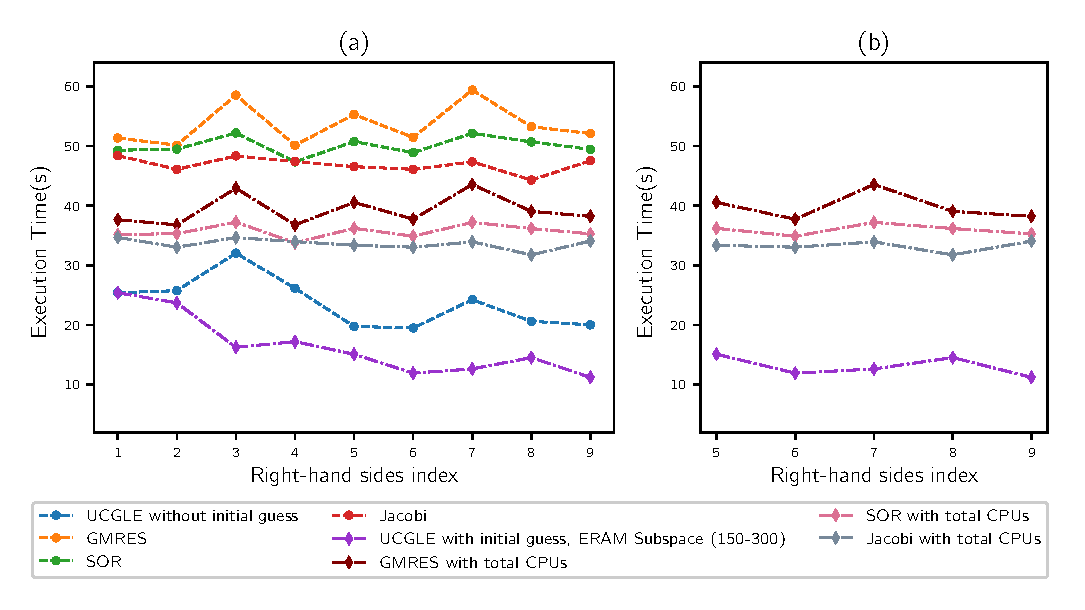
\includegraphics[width=6.4in]{fig/seqrhs3.eps}
	\caption{$Mat2$: time comparison for solving a sequence of linear systems. (a) shows the solution time for 9 sequent linear systems; (b) shows the cases extracted from (a) after the good selection of parameters in UCGLE.}
	\label{fig:seqrhs3}
\end{figure}

\begin{table}[htbp]
	\small
	\label{tb3}
	\caption{$Mat2$:  iterative step comparison for solving a sequence of linear systems.}
	\centering
	\renewcommand{\arraystretch}{1.6}
	\begin{tabular}{c*{9}{c}}
		\toprule
		\cellcolor{gray!50}Method              & \cellcolor{gray!50}1 &  \cellcolor{gray!50}2 &  \cellcolor{gray!50}3 &  \cellcolor{gray!50}4 &  \cellcolor{gray!50}5  &  \cellcolor{gray!50}6  & \cellcolor{gray!50}7 & \cellcolor{gray!50}8 & \cellcolor{gray!50}9\\
		\midrule
		GMRES & 1316	&1277	&1460	&1278	&1409	&1325	&1472	&1369	&1342\\
			\cellcolor{gray!20}GMRES+SOR            & 	\cellcolor{gray!20}1197&		\cellcolor{gray!20}1219&		\cellcolor{gray!20}1336&		\cellcolor{gray!20}1173	&	\cellcolor{gray!20}1290	&	\cellcolor{gray!20}1194	&	\cellcolor{gray!20}1335	&	\cellcolor{gray!20}1289	&	\cellcolor{gray!20}1213\\
		GMRES+Jacobi            & 1278&	1185	&1283&	1220	&1191&	1184	&1218&	1159&	1239\\
			\cellcolor{gray!20}UCGLE w/o initial guess     & 	\cellcolor{gray!20}666	&	\cellcolor{gray!20}671	&	\cellcolor{gray!20}831	&	\cellcolor{gray!20}689	&	\cellcolor{gray!20}701	&	\cellcolor{gray!20}685	&	\cellcolor{gray!20}837	&	\cellcolor{gray!20}736	&	\cellcolor{gray!20}714\\
		UCGLE with initial guess     & 666	&595	&470	&491	&544	&464	&485	&532	&440\\
		\hline
	\end{tabular}
\end{table}

For the tests of $Mat3$, the GMRES restart size is $150$, and the Krylov subspace size of ERAM Components keeps the same to be $200$. Meanwhile, for the 2nd, 3rd and 4th linear systems, the parameter $l'$ of initial guess are respectively $20$, $30$ and $40$, for the remaining linear systems, this parameter keeps $40$. For the solving the linear systems by UCGLE with an initial guess, we can find that with the augmentation of $l'$, the iteration numbers for the first four linear systems decrease quickly from $360$ to $283$ with approximately $1.3 \times$ speedup. For $Mat3$, SOR preconditioned GMRES is already good, but UCGLE with initial guess has still about $2.2 \times$ speedup of convergence. Even in the case that the computing unit number of SOR preconditioned GMRES equals the total number of UCGLE, UCGLE with initial guess can achieve $2.2 \times$ of execution time speedup. With the augmentation of the parameter $l'$, there will be a strong impact on the convergence. Since the $Mat3$ is generated with the clustered eigenvalues which are randomly distributed inside a fixed region of the real-imaginary plan, if $l'$ is larger, it can be seen as there are much more eigenvalues generated, even they are not very accurate compared with the real ones. The inaccuracy of eigenvalues can result in the enlargement the norm in Equation (\ref{rnk2}), but it can still very quickly converge. It is effective to generate an initial guess vector with very large $l'$, but not the same case for the parameter $l$ inside each preconditioning, since the too many times of repeats for each time restart will amplify quicky this inaccuracy of norm, and it is easy to result in the difficulties of convergence.

In order to use UCGLE for solving a large number of linear systems in sequence, it is necessary to choose the suitable parameters by the evaluation of a small number of sequent linear systems. After the selection of parameters, we compare the best cases of each method with the least time consumption. The results for three test matrices are shown in Fig. \ref{fig:seqrhs1} (b), Fig. \ref{fig:seqrhs2} (b) and Fig. \ref{fig:seqrhs3} (b). We conclude that for $Mat1$, UCGLE with initial guess has about $4.4\times$ for the acceleration of convergence and $1.7\times$ for the speedup of execution time. For $Mat2$, it has about $2.6\times$ acceleration for the convergence and $4.3\times$ for the speedup of time. For $Mat3$, it has about $3.2\times$ acceleration for the convergence and $2.0\times$ for the speedup of time. 

\begin{figure}[htbp]
	\centering
	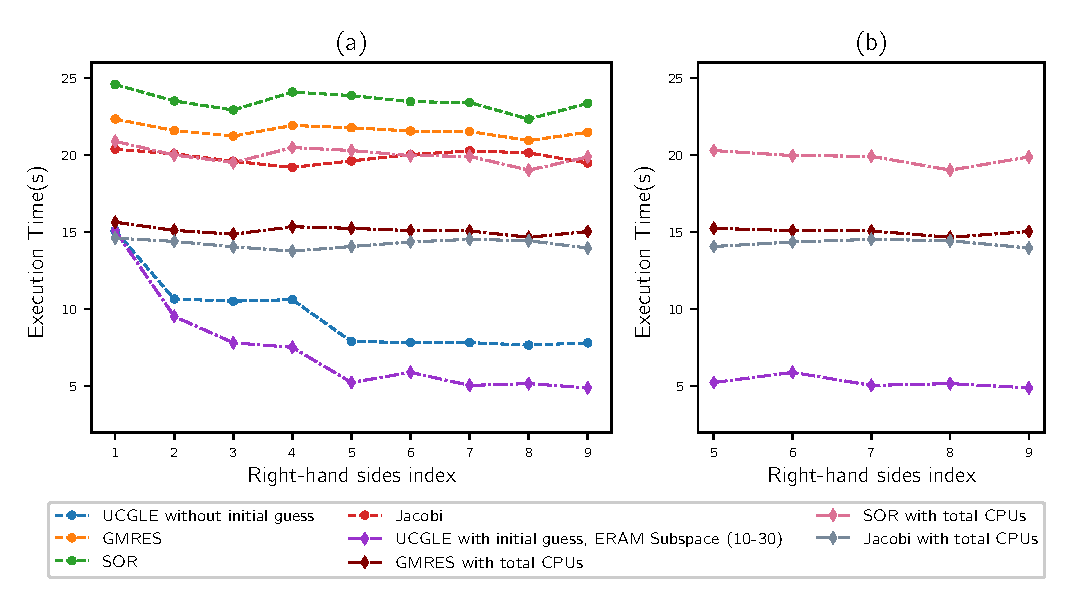
\includegraphics[width=6.4in]{fig/seqrhs2.eps}
	\caption{$Mat3$: time comparison for solving a sequence of linear systems. (a) shows the solution time for 9 sequent linear systems; (b) shows the cases extracted from (a) after the good selection of parameters in UCGLE.}
	\label{fig:seqrhs2}
\end{figure}

%UCGLE with initial guess     & 5456 & 91 & 253 & 112 & 121 & 218  & 183 & 120 & 109\\
%UCGLE w/o initial guess     & 5456 & 5114 & 5702 & 5750 & 5670 &5699 &5387&5506& 5195\\
\begin{table}[htbp]
	\small
	\label{tb2}
	\caption{$Mat3$: iterative step comparison for solving a sequence of linear systems.}
	\centering
	\renewcommand{\arraystretch}{1.6}
	\begin{tabular}{c*{9}{c}}
		\toprule
		\cellcolor{gray!50}Method              & \cellcolor{gray!50}1 &  \cellcolor{gray!50}2 &  \cellcolor{gray!50}3 &  \cellcolor{gray!50}4 &  \cellcolor{gray!50}5  &  \cellcolor{gray!50}6  & \cellcolor{gray!50}7 & \cellcolor{gray!50}8 & \cellcolor{gray!50}9\\
		\midrule
		GMRES & 914 & 912 & 892 &885  & 895 & 905  &911&892& 904\\
		\cellcolor{gray!20}GMRES+SOR            & 	\cellcolor{gray!20}895 & 	\cellcolor{gray!20}871 & 	\cellcolor{gray!20}856 & 	\cellcolor{gray!20}885 & 	\cellcolor{gray!20}879 & 	\cellcolor{gray!20}870 &	\cellcolor{gray!20}868&	\cellcolor{gray!20}838&	\cellcolor{gray!20}868\\
		GMRES+Jacobi            & 894 & 888 & 875 & 864 & 876 & 887 &892&888&872\\
			\cellcolor{gray!20}UCGLE w/o initial guess     & 	\cellcolor{gray!20}673 & 	\cellcolor{gray!20}364 & 	\cellcolor{gray!20}355 & 	\cellcolor{gray!20}360 & 	\cellcolor{gray!20}367 &	\cellcolor{gray!20}363 &	\cellcolor{gray!20}363&	\cellcolor{gray!20}351& 	\cellcolor{gray!20}364\\
		UCGLE with initial guess     & 673 & 396 & 291 & 283 & 339 & 338  & 274 & 279 & 267\\
		\hline
	\end{tabular}
\end{table}

\subsubsection{Analysis and Conclusions}

In conclusion, the UCGLE, especially it with the recycling eigenvalues to generate initial guess vector using the eigenvalues, can significantly accelerate the convergence and reduce the time consumption for solving a sequence of linear systems. However, the time employed by the LS iterative recurrence, especially a small number of Sparse Matrix-Vector Product operations inside makes the time speedup not consistent with the convergence speedup. For example, in Table 3, UCGLE with initial guess has almost $3.0 \times$ acceleration on the convergence over the classic GMRES for solving the 3rd linear system. However, it has only about $2.0 \times$ acceleration on the performance in the case that the classic GMRES and GMRES Component inside UCGLE have the same number of computing units. It is caused by the recurrence of LS iterations to perform the preconditioning on GMRES Component after receiving the parameters from LS Component. Nevertheless, UCGLE is more efficient to solve the sequences of linear systems, and with its distributed and parallel communication framework, it is a good candidate for solving non-Hermitian linear systems in sequence on much larger machines.

\section{Conclusion}

\clearemptydoublepage